\documentclass{../grid-link-report}

\SetClassAssetsDir{../class-assets}
\newcommand{\projectassetsdir}{../project-assets}
\project{Clements Gap BESS}
\client{Enzen}
\developer{Pacific Blue (formerly Pacific Hydro)}
\title{Voltage Control Strategy}
\docnumber{HEYWOODBESS-GR-RPT-013}
\issueddate{16 May 2025}
\revision{1-0-0}
\revisionhistorycsvpath{report-assets/revision-history.csv}
\clientlogopath{\projectassetsdir/client-logo.png}
\usepackage{pdflscape}   % For landscape pages
\usepackage{graphicx}
\usepackage{enumitem}
\usepackage{multirow}
\usepackage{pgfplotstable} % For reading and displaying tables from CSV files
\usepackage{booktabs}      % For better-looking tables
\usepackage[acronym]{glossaries}



\begin{document}
	% Draft commands
	%\listoftodos
	\frontmatter
	\maketitle
	%\adddraftstamp
	
	\makedisclaimer
	\clearpage
	\tableofcontents
	\makerevisionhistorypage
	%\makeaboutgridlink
	
	\mainmatter
	
	\chapter{Summary of Voltage Control Strategy}

	The Heywood Battery Energy Storage System (HEYWOODBESS) is a $\pm~285MW/1140MWh$ Battery Energy Storage Project, located 5 km from the town of Heywood and 300 km west of Melbourne in Victoria. As part of this project, the new  275kV underground line will be constructed between HEYWOODBESS site and existing 275 kV switchyard.
	
	\ac{HEYWOODBESS} will include include 92 SMA Sunny Central 4.6 MW (SCS 4600 UP-S) inverters which will be connected to two 275/33kV, 160MVA transformers through the 33kV reticulation system. Each inverter will have a dedicated 33/0.69kV, 4.6 MVA step up transformer. .
	
	\ac{HEYWOODBESS} will operate in voltage droop control mode by default, controlling the 275kV connection point with a 4\% droop on a 112.575 MVAr base.
	
	The proposed maximum capacity of HEYWOODBESS at the connection point is $\pm$ 285 MW at ambient air temperatures between 35°C and 50°C. 
	
	{
	\thicktablelines
	\begin{longtable}{|C{5cm}|C{10cm}|} 
		\caption{Connection Overview}
		\label{tab:connection-overview}
		\\	
		\toprule
		
		\rowcolor{tableheaderblue}
		\bfseries \color{white}Connection Overview & \bfseries \color{white}Description\\
		\endhead
		\bottomrule \endfoot
		\csvreader[
		separator=semicolon,
		late after line=\\\hline,
		late after last line=,
		before reading={\catcode`\#=12},
		after reading={\catcode`\#=6}]%
		{report-assets/connection_overview.csv}{1=\CSVOverview,2=\CSVDescription}{\CSVOverview & \CSVDescription}
		\\\hline
	\end{longtable}
	}
	
	\ac{HEYWOODBESS} uses as closed loop PID controller - the FLUENCE Power Plant Controller (PPC), to control the point of connection to desired active and reactive power setpoints. The \ac{PPC} receives these setpoints from the sites's Energy Management System(EMS) controller and dispatches the battery inverters accordingly. The power quality meter providing feedback to the PPC receives its current transformer (CT) inputs from CTs located at the high voltage side of the main transformer while voltage transformer (VT) inputs are from a VT located on AusNet side of the projects delineation boundary.
	


	\chapter{Remote Voltage Control}
		
	{
	\thicktablelines
	\begin{longtable}{|C{2cm}|C{3cm}||C{6cm}|C{4cm}|} 
		\caption{Reference Change Series of Events}
		\label{tab:remote-voltage-control}
		\\	
		\toprule
		
		\rowcolor{tableheaderblue}
		\bfseries \color{white}Action & \bfseries \color{white}By  & \bfseries \color{white}Description  & \bfseries \color{white}Response By\\
		\endhead
		\bottomrule \endfoot
		\csvreader[
		separator=semicolon,
		late after line=\\\hline,
		late after last line=,
		before reading={\catcode`\#=12},
		after reading={\catcode`\#=6}]%
		{report-assets/voltage_control.csv}{1=\CSVAction,2=\CSVBy,3=\CSVDescription,4=\CSVResponseBy}{\CSVAction &\CSVBy&\CSVDescription&\CSVResponseBy}
		\\\hline
	\end{longtable}
	}		
	The \ac{PPC} receives the voltage setpoint signal from the site's EMS - which is responsible for triaging setpoints received from various sources eg. NSP, AEMO, the dispatch system or the plant operator.	Once a setpoint is received, the controller calculates a droop adjusted reactive power target based on the error between the measured voltage at the POC and the voltage reference setpoint. The controller then issues a reactive power target to each inverter based on the error between the measured reactive power output and the droop adjusted reactive power reference.
	
	The relationship between the droop adjusted reactive power reference and the error between the voltage reference and the measured voltage at the POC ($V_{error,poc}$) is given by the chart below. This characteristic reflects a 2\% voltage droop on a reactive power base of 23.7 MVAr. Therefore, we expect that the generating system will target a reactive power output of $\pm$ 23.7 MVAr whenever $|V_{poc}-V_{vref}| \geq 0.02 $.
	
	\begin{figure}[H]
		\centering
		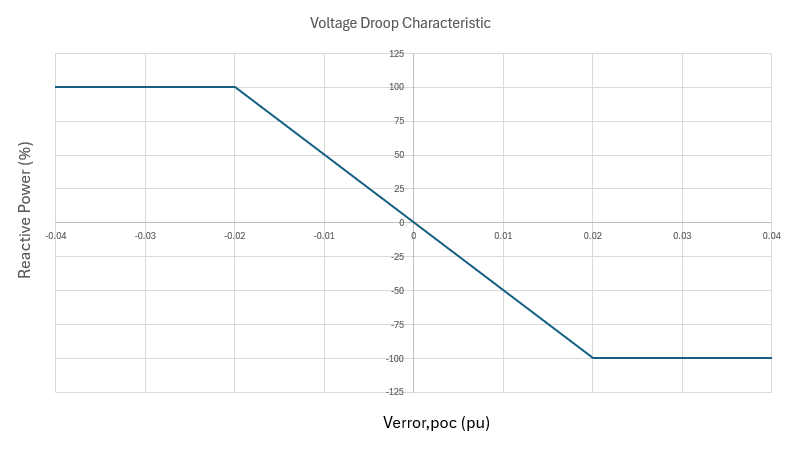
\includegraphics[width=0.9\linewidth]{report-assets/voltage-droop-char.png}
		\caption{CG BESS Voltage Droop Characteristic}
		\label{fig:vdroop-char}
	\end{figure}
		
	\chapter{Remote PF Control}
	{
	\thicktablelines
	\begin{longtable}{|C{2cm}|C{3cm}||C{6cm}|C{4cm}|} 
		\caption{PF Reference Change Series of Events}
		\label{tab:remote-pf-control}
		\\	
		\toprule
		
		\rowcolor{tableheaderblue}
		\bfseries \color{white}Action & \bfseries \color{white}By  & \bfseries \color{white}Description  & \bfseries \color{white}Response By\\
		\endhead
		\bottomrule \endfoot
		\csvreader[
		separator=semicolon,
		late after line=\\\hline,
		late after last line=,
		before reading={\catcode`\#=12},
		after reading={\catcode`\#=6}]%
		{report-assets/pf_control.csv}{1=\CSVAction,2=\CSVBy,3=\CSVDescription,4=\CSVResponseBy}{\CSVAction &\CSVBy&\CSVDescription&\CSVResponseBy}
		\\\hline
	\end{longtable}
	}		
	The \ac{PPM} receives the voltage setpoint signal from the site's EMS - which is responsible for triaging setpoints received from various sources eg. NSP, AEMO, the dispatch system or the plant operator.	Once a power factor setpoint is received, the controller calculates a reactive power target based on the measured active power and the power factor setpoint. The controller then issues a reactive power target to each inverter based on the error between the measured reactive power output and reactive power reference.
	
	
	
	\chapter{Remote Reactive Power Control}
	{
	\thicktablelines
	\begin{longtable}{|C{2cm}|C{3cm}||C{6cm}|C{4cm}|} 
		\caption{Reactive Power Reference Change Series of Events}
		\label{tab:remote-q-control}
		\\	
		\toprule
		
		\rowcolor{tableheaderblue}
		\bfseries \color{white}Action & \bfseries \color{white}By  & \bfseries \color{white}Description  & \bfseries \color{white}Response By\\
		\endhead
		\bottomrule \endfoot
		\csvreader[
		separator=semicolon,
		late after line=\\\hline,
		late after last line=,
		before reading={\catcode`\#=12},
		after reading={\catcode`\#=6}]%
		{report-assets/q_control.csv}{1=\CSVAction,2=\CSVBy,3=\CSVDescription,4=\CSVResponseBy}{\CSVAction &\CSVBy&\CSVDescription&\CSVResponseBy}
		\\\hline
	\end{longtable}
	}		
	When in Reactive Power Control (Q Control), the \ac{PPM} may receive a change in reactive power setpoint via the site's EMS - which is responsible for triaging setpoints received from various sources eg. NSP, AEMO, the dispatch system or the plant operator.	Once a reactive power setpoint is received, the controller then issues a reactive power target to each inverter based on the error between the measured reactive power output and reactive power reference. The reactive power output at the point of connection is limited to $\pm$ 23.7 MVAr.


	\chapter{Reactive Power Capability}
	
	Clements Gap BESS is capable of providing $\pm$ 23.7 MVAr ($0.395 * P_{base}$) at the generating system point of connection, for active power outputs of $\pm$ 60 MW and ambient air temperatures up to $50^{\circ}\text{C}$. This is demonstrated by the reactive capability curves below. This assessment has considered continuous uninterrupted operation and whether the inverters are capable of providing sufficient reactive power at steady state for voltage disturbance steps from 1.0 - 1.1 pu and 1.0 - 0.9 pu at the point of connection.

	\begin{figure}[H]
		\centering
		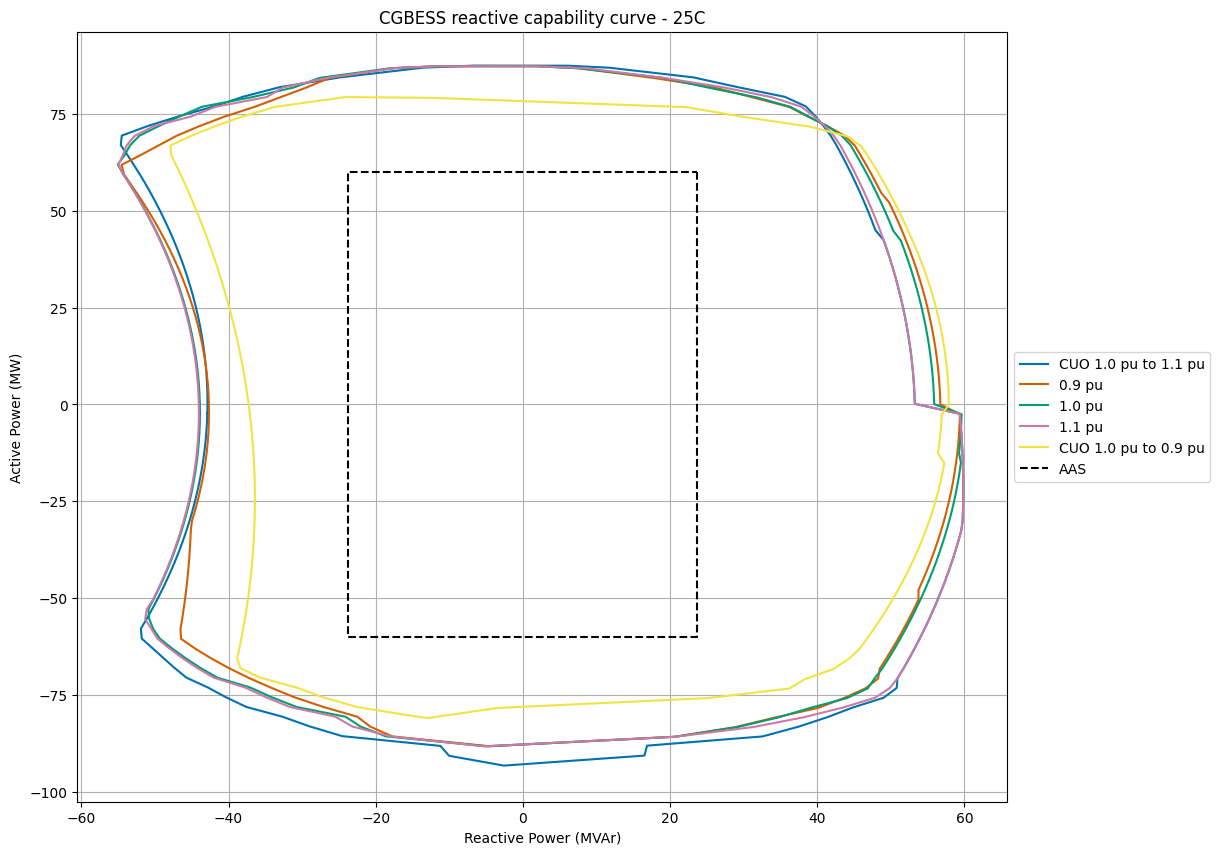
\includegraphics[width=0.9\linewidth]{report-assets/reactive capability curve - 25C.png}
		\caption{CG BESS Reactive Capability Curve at $25^\circ$C}
		\label{fig:q-capability-25degc}
	\end{figure}

	\begin{figure}[H]
		\centering
		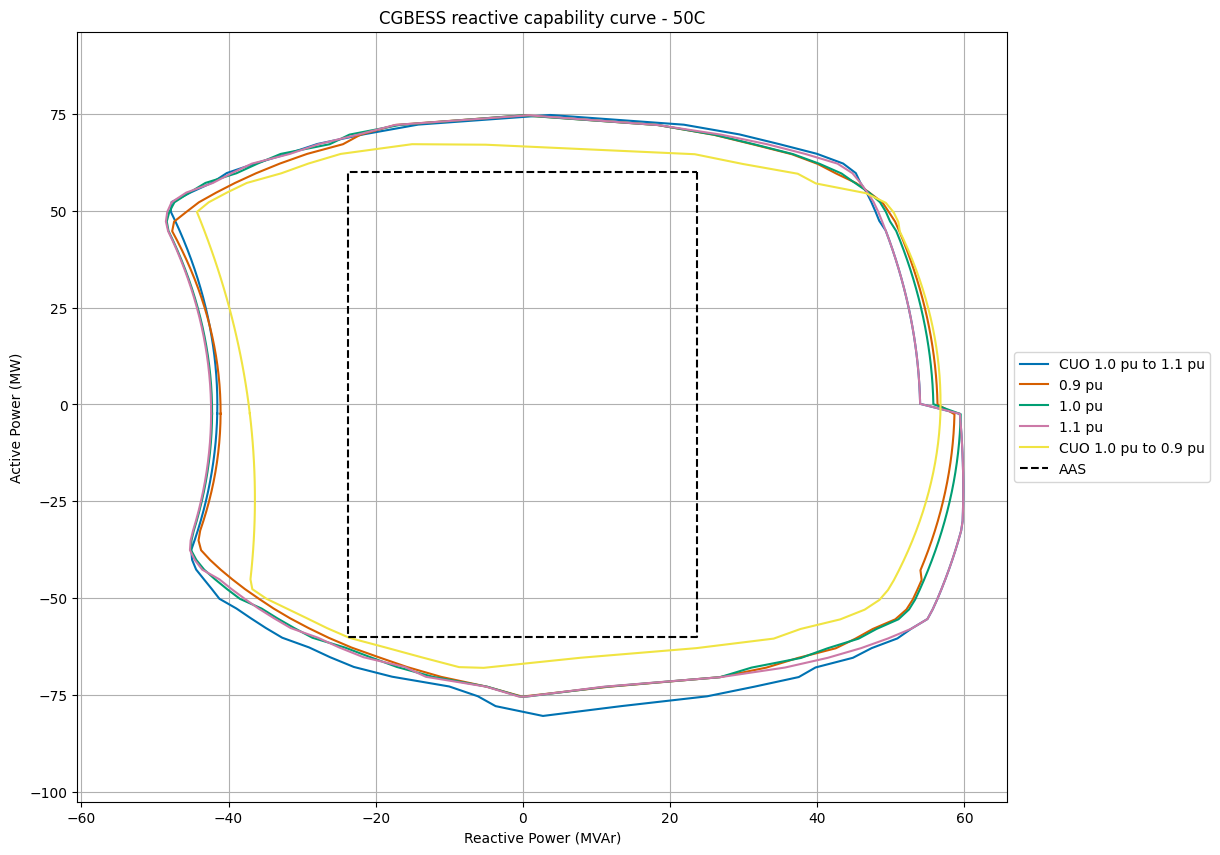
\includegraphics[width=0.9\linewidth]{report-assets/reactive capability curve - 50C.png}
		\caption{CG BESS Reactive Capability Curve at $50^\circ$C}
		\label{fig:q-capability-50degc}
	\end{figure}
	
	The capability of the generating system at the POC was determined as a function of the individual capability of the SMA SCS 3600 UP inverters. These have been provided for reference below.
	
	\begin{figure}[H]
		\centering
		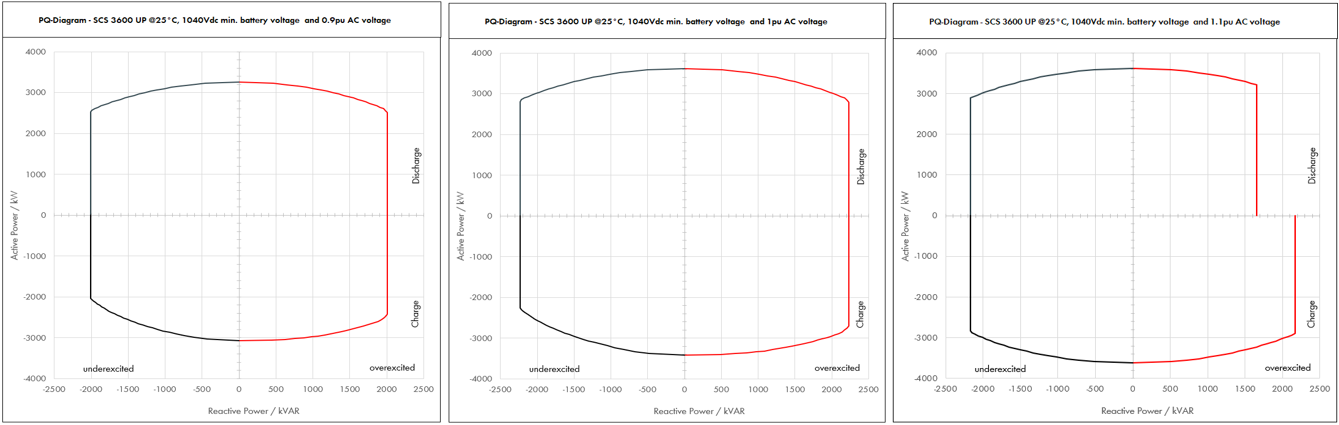
\includegraphics[width=1.0\linewidth]{report-assets/inv-q-cap-25degC.png}
		\caption{SMA SCS 3600 UP Reactive Capability Curve by terminal voltage at $25^{\circ}\text{C}$}
		\label{fig:inv-q-capability-25degc}
	\end{figure}	

	\begin{figure}[H]
		\centering
		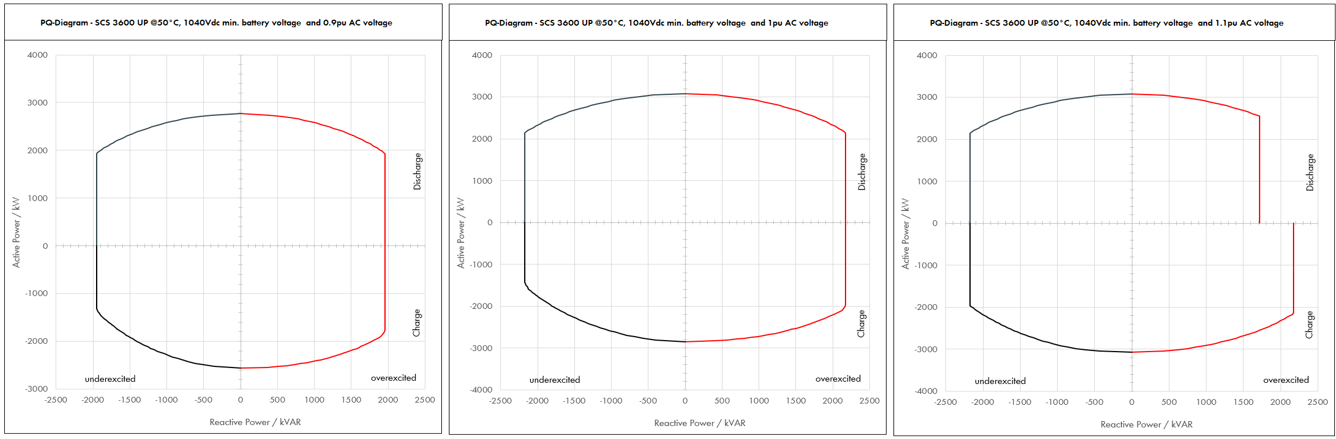
\includegraphics[width=1.0\linewidth]{report-assets/inv-q-cap-50degC.png}
		\caption{SMA SCS 3600 UP Reactive Capability Curve by terminal voltage at $50^{\circ}\text{C}$}
		\label{fig:inv-q-capability-50degc}
	\end{figure}	
	
	\chapter{Physical Equipment}
	The substation single line diagram (SLD) is illustrated in Figure \ref{fig:substation-sld}. This diagram outlines the electrical configuration of primary plant as well as the CTs and VTs used for metering.
	
	Significant primary plant for this generating system are as follows
	\begin{itemize}
		\item{1 x 132kV/33kV 70 MVA main transformer}
		\item{5 x 33kV collector feeders}
		\item{25 x SMA SCS 3600 UP inverters}
		\item{2 x 33kV HF filter banks (12MVAr + 3 MVAr)}
		\item{5 x 500 kVA collector auxiliary transformers}
		\item{1 x 315 kVA auxiliary transformer}
		
	\end{itemize}
	
	\begin{landscape}
		\begin{center}
			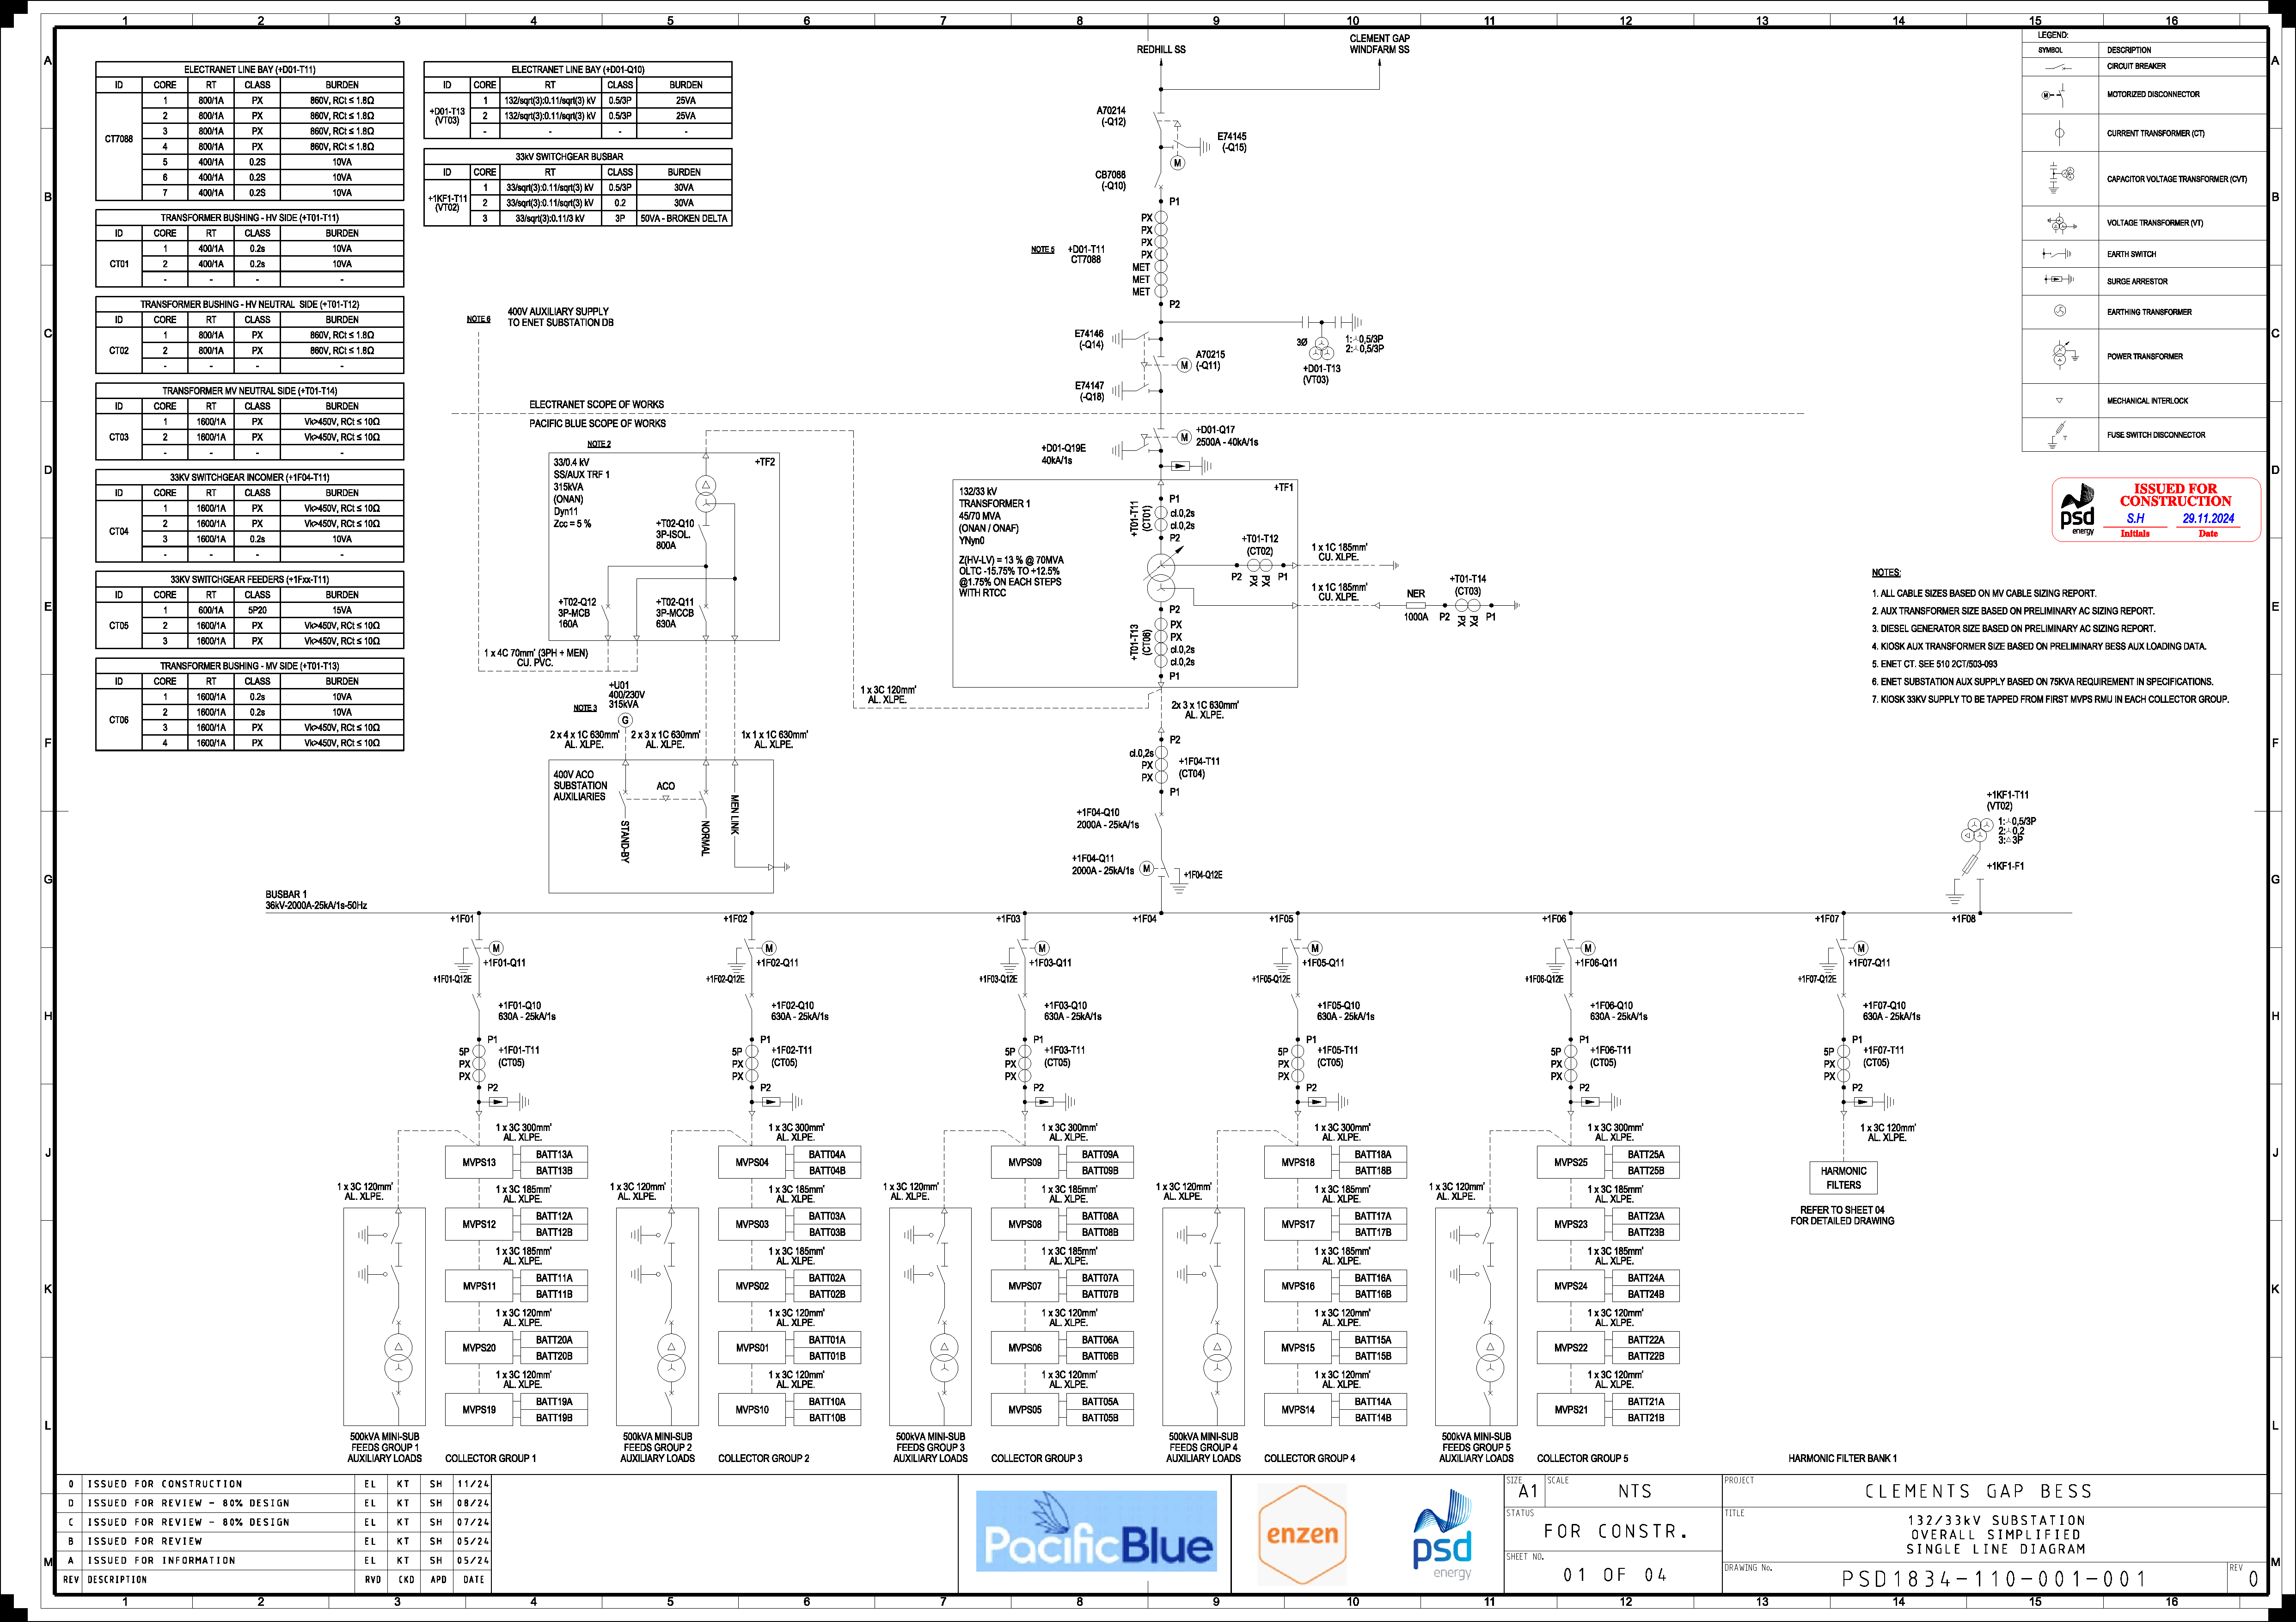
\includegraphics[width=\linewidth]{References/PSD1834-110-001-001.pdf}
			\label{fig:substation-sld}
		\end{center}
	\end{landscape}
	
	\chapter{Transformers}
		\section{Inverter Transformers}
		Clements Gap Bess contains twenty five (25) 3.6 MVA 33/0.63 kV three-phase two-winding inverter transformers with parameters given in Table \ref{tab:inverter-transformer}. These transformers are fitted with an off-load tap changer and are typically configured at the nominal tap position. Please refer to \cite{mvps-sld} which illustrates the electrical configuration of the medium voltage power station. Please refer to the medium voltage transformer datasheet \cite{mvt-datasheet}.
		
		{
		\thicktablelines
		\begin{longtable}{|C{6cm}|C{4cm}|} 
			\caption{3.78 MVA Inverter Transformer Details}
			\label{tab:inverter-transformer}
			\\	
			\toprule
			
			\rowcolor{tableheaderblue}
			\bfseries \color{white}Parameter & \bfseries \color{white}Value\\
			\endhead
			\bottomrule \endfoot
			\csvreader[
			separator=semicolon,
			late after line=\\\hline,
			late after last line=,
			before reading={\catcode`\#=12},
			after reading={\catcode`\#=6}]%
			{report-assets/inverter_transformer.csv}{1=\CSVParameter,2=\CSVValue}{\CSVParameter &\CSVValue}
			\\\hline
		\end{longtable}
		}				
		
		
		\section{Main Transformer}
		Clements Gap Bess contains a single 70 MVA three-phase two-winding main transformer with parameters given in Table \ref{tab:main-transformer}. This transformer is fitted with an on-load tap changer (OLTC) with seventeen (17) taps, where the nominal tap is tap 10 (1.0 pu). Please refer to the datasheet for the main transformer \cite{main-tx-datasheet} and the substation sld \cite{substation-sld} which illustrates the electrical configuration of the main transformer.
		
		
		{
			\thicktablelines
			\begin{longtable}{|C{6cm}|C{4cm}|} 
				\caption{70 MVA Main Transformer Details}
				\label{tab:main-transformer}
				\\	
				\toprule
				
				\rowcolor{tableheaderblue}
				\bfseries \color{white}Parameter & \bfseries \color{white}Value\\
				\endhead
				\bottomrule \endfoot
				\csvreader[
				separator=semicolon,
				late after line=\\\hline,
				late after last line=,
				before reading={\catcode`\#=12},
				after reading={\catcode`\#=6}]%
				{report-assets/main_transformer.csv}{1=\CSVParameter,2=\CSVValue}{\CSVParameter &\CSVValue}
				\\\hline
			\end{longtable}
		}
		
	The OLTC voltage set point is expected to be set to a fixed value of 1.0 pu, independent of the level of generation. The OLTC auto-voltage regulation (AVR) relay utilises a dead band ensuring that the target is achieved to within $\pm$ 0.015 pu. An initial tap change in response to a voltage deviation beyond the control dead band is undertaken after a defined delay of 10 seconds. This is commonly understood as an AVR constant time program. If after a single tap change operation the voltage is still outside the deadband, another tap will be expected after an additional ten seconds. This delay of ten seconds is representative of the total tapping time - that is it includes any mechanical delays of the OLTC and wait times configured in the AVR. This time delay has been selected to ensure no unwanted interference between primary and secondary control loops while ensuring it is fast enough to ensure the generator maintains continuous uninterrupted operation for a variety of network disturbances. Please refer to the TAPCON 230 AVR manual \cite{avr-manual} and OLTC switching datasheet provided \cite{oltc-switching}.   		
	\chapter{Reactive Plant}
	
	As part of R1 a harmonic emissions assessment has been undertaken and two C-Type filter banks have been proposed in order to address harmonic emmissions at the point of connection and to ensure compliance with S5.2.5.2 of the generator performance standard. These filters are connected to the 33kV bus and supply a total of 15 MVArs of passive reactive power when in service. Please refer to the harmonic emissions assessment \cite{harmonic-assessment} and substation sld \cite{substation-sld} which details the connection point of the filter banks.
	
	{
	\thicktablelines
	\begin{longtable}{|C{2cm}|C{3cm}|C{4cm}|C{3cm}|C{3cm}|} 
		\caption{C-Type Filter Details}
		\label{tab:harmonic-filters}
		\\	
		\toprule
		
		\rowcolor{tableheaderblue}
		\bfseries \color{white}Name & \bfseries \color{white}Type & \bfseries \color{white}Rated Reactive Power & \bfseries \color{white}Tuning Order & \bfseries \color{white}Quality Factor\\
		\endhead
		\bottomrule \endfoot
		\csvreader[
		separator=semicolon,
		late after line=\\\hline,
		late after last line=,
		before reading={\catcode`\#=12},
		after reading={\catcode`\#=6}]%
		{report-assets/filter_specs.csv}{1=\CSVName,2=\CSVType,3=\CSVRatedPower,4=\CSVTuningOrder,5=\CSVQualityFactor}{\CSVName & \CSVType & \CSVRatedPower & \CSVTuningOrder & \CSVQualityFactor}
		\\\hline
	\end{longtable}
	}	
	
	
	
	
	\chapter{Control Block Diagram}
	Detailed control block diagrams have been provided directly to AEMO by SMA as they are confidential in nature.
	\chapter{Control Mode Switching}
	Clements Gap BESS is capable of operating in three main reactive power control modes
	
	\begin{enumerate}
		\item Voltage droop control
		\item Power factor control
		\item Reactive power control
	\end{enumerate}
	
	The generating system EMS is responsible for ensuring that switching between these modes, whether by a local operator or remote party, is bumpless - that is to say that there will not be large changes in reactive power output (resulting in voltage steps) when transitioning between reactive power modes.
	
	Please refer to the SCADA Control Philosophy \cite{scada-philo} for a summary of the CG BESS control system design and the active and reactive power AEMO/TNSP control schemes applicable to this site.
	
	\begin{figure}[H]
		\centering
		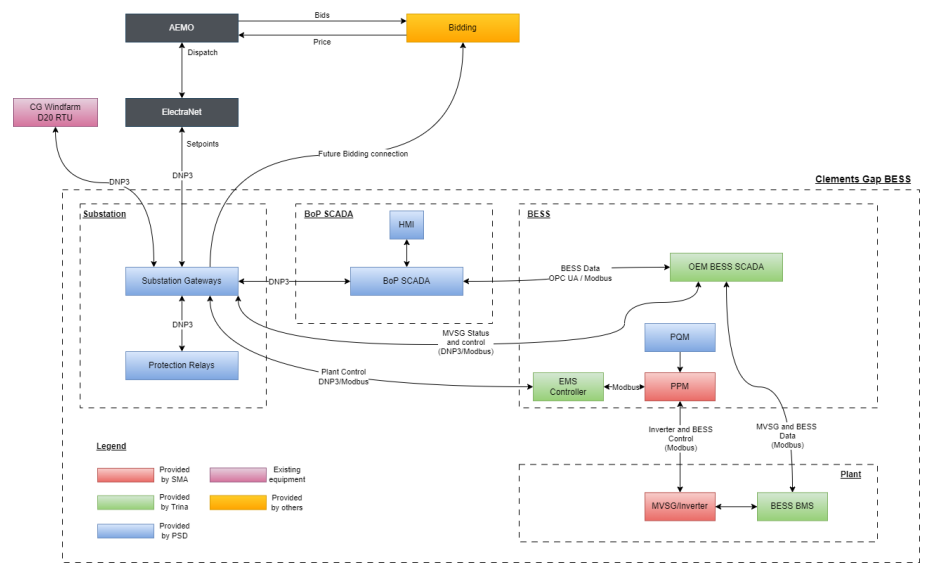
\includegraphics[width=1.0\linewidth]{report-assets/control-flow-overview.png}
		\caption{Control Scheme Overview}
		\label{fig:control-scheme-flow}
	\end{figure}	
	
	
	\chapter{Inverter Level Controls}
	The inverters at Clements Gap BESS are equipped with a voltage-dependent reactive power control (CArCtlVol) mode. This voltage control scheme allows the inverters to provide additional reactive power based on the inverter AC voltage. This mode supports an external set point $\it{VolNomSpt}$ that will effectively shift the Q-V characteristic left-ward or right-ward. The Q-V characteristic for this mode with a voltage setpoint of 1.0pu has been included below. For this site, the AC voltage setpoint is initialised with a value of 1.0 pu (as per the parameters $\it{VArCtlVol\_VolNomSptMod}$ and $\it{VArCtlVol\_VolNomSptInit}$). Please refer to the PSCAD RUG included in the R1 package for more details on these parameters. 
	
	
	\begin{figure}[H]
		\centering
		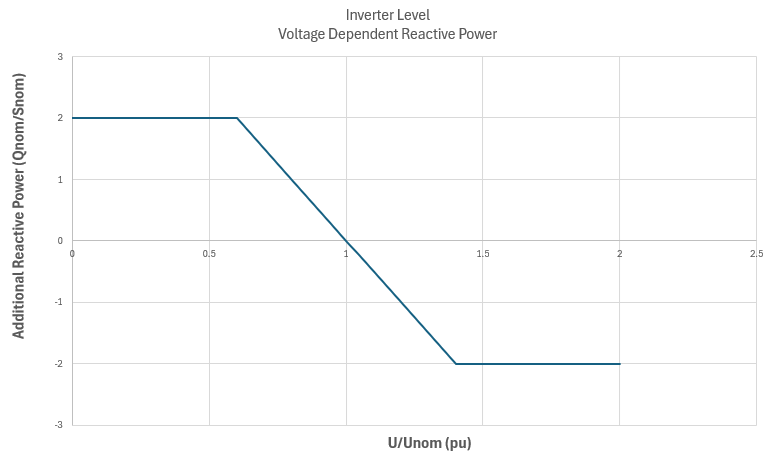
\includegraphics[width=1.0\linewidth]{report-assets/inverter-level-voltage-control_char.png}
		\caption{Inverter Level Voltage Dependent Reactive Power}
		\label{fig:inverter-level-voltage-control_char}
	\end{figure}		
	
	\chapter{Signal List}
	Please refer to the AEMO IO Schedule \cite{aemo-io}. This document details the input/output (IO) signals shared between CG BESS and AEMO/ElectraNet.
	
	\chapter{SCADA, Communication and Latency}
	For additional information on 
	\begin{enumerate}
		\item the applicable control schemes,
		\item pathways for control setpoints,
		\item heartbeat and communications fail detection
		\item availability requirements of the control system
	\end{enumerate}
	
	please refer to the SCADA Control Philosophy \cite{scada-philo}.
	
	For additional information on the communication network layout please refer to the Communication Architecture diagram \cite{comms-arch}. Please note that the site's communication latency is going to be measured and documented during commissioning.
	
	
	
	\chapter{Generating System HMI}
	The SCADA servers providing the Human Machine Interface (HMI) for this project are specified in Table \ref{tab:servers}.
	{
	\thicktablelines
	\begin{longtable}{|C{3cm}|C{5cm}|} 
		\caption{SCADA Server Details}
		\label{tab:servers}
		\\	
		\toprule
		
		\rowcolor{tableheaderblue}
		\bfseries \color{white}Type & \bfseries \color{white}Function\\
		\endhead
		\bottomrule \endfoot
		\csvreader[
		separator=semicolon,
		late after line=\\\hline,
		late after last line=,
		before reading={\catcode`\#=12},
		after reading={\catcode`\#=6}]%
		{report-assets/scada_servers.csv}{1=\CSVType,2=\CSVFunction}{\CSVType & \CSVFunction}
		\\\hline
	\end{longtable}
	}
	
	An example of the interface being developed for this project has been provided in the figure below.
	
	\begin{figure}[H]
		\centering
		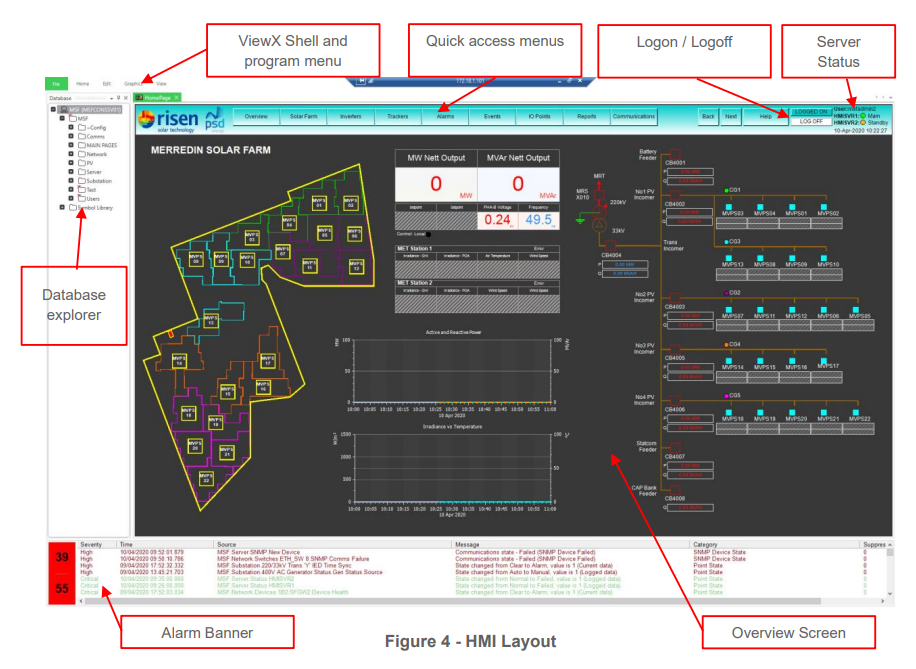
\includegraphics[width=1.0\linewidth]{report-assets/SCADA-HMI.png}
		\caption{Example of the HMI}
		\label{fig:scada-hmi}
	\end{figure}
	
	Please refer to the SCADA Functional Specification \cite{scada-spec} for more information on the HMI functional requirements, various interfaces and symbol conventions.


	\chapter{Protection Functionality}
	Please refer to the Protection Setting Report \cite{protection-settings-report} which outlines the protection functions for the site including for the harmonic filters, transformers and 33kV bus.
	
	Please refer to the PSCAD Releasable User Guide (RUG) for the inverter protection settings used for this project.
	

	\chapter*{Acronyms}
\begin{acronym}%[JSONP]\itemsep0pt
	\acro{AAS}{Automatic Access Standard}
	\acro{AEMO}{Australian Energy Market Operator}
	\acro{VSL}{Voltage Stackable Logic}
	\acro{AGC}{Automatic Generation Control}
	\acro{AVR}{Automatic Voltage Regulator}
	\acro{BESS}{Battery Energy Storage System}
	\acro{BOP}{Balance Of Plant}
	\acro{CGBESS}{Clements Gap BESS}
	\acro{Heywood BESS}{Heywood Battery Energy Storage System}	
	\acro{CSR}{Connection Studies Report}
	\acro{CT}{Current Transformer}
	\acro{CUO}{Continuous Uninterrupted Operation}
	\acro{HV}{High Voltage}
	\acro{DMAT}{Dynamic Model Acceptance Test}
	\acro{DYR}{PSSE Dynamics Data File}
	\acro{EMT}{Electromagnetic Transients}
	\acro{FIA}{Full Impact Assessment}
	\acro{FRT}{Fault Ride-Through}
	\acro{GPS}{Generator Performance Standards}
	\acro{HVRT}{High Voltage Ride-Through}
	\acro{LV}{Low Voltage}
	\acro{LVRT}{Low Voltage Ride-Through}
	\acro{MV}{Medium Voltage}
	\acro{NEM}{National Electricity Market}
	\acro{NSP}{Network Service Provider}
	\acro{OEM}{Original Equipment Manufacturer}
	\acro{OFRT}{Over-Frequency Ride-Through}
	\acro{OLTC}{On-Load Tap Changer}
	\acro{OPDMS}{Operations and Planning Data Management System}
	\acro{OVRT}{Over-Voltage Ride-Through}
	\acro{PLL}{Phase-Locked Loop}
	\acro{PLR}{Partial Load Rejection}
	\acro{PPC}{Power Plant Controller}
	\acro{PPM}{Power Plant Manager}
	\acro{RoCoF}{Rate of Change of Frequency}
	\acro{RMS}{Root Mean Square}
	\acro{RMU}{Ring Main Unit}
	\acro{RUG}{Releasable User Guide}
	\acro{S5251}{Reactive Power Capability}
	\acro{S5254}{Generating System Response to Voltage Disturbances}
	\acro{SCR}{Short Circuit Ratio}
	\acro{SMIB}{Single Machine, Infinite Bus}
	\acro{SLD}{Single Line Diagram}
	\acro{TOV}{Temporary Over-Voltage}
	\acro{UFRT}{Under-Frequency Ride-Through}
	\acro{UVRT}{Under-Voltage Ride-Through}
	\acro{VCS}{Voltage Control Strategy}
	\acro{WAN}{Wide Area Network}
	\acro{WF}{Wind Farm}
	\acro{VOIP}{Voice Over Internet Protocol}
	\acro{VRR}{Voltage Regulation Relay}
	\acro{VT}{Voltage Transformer}
\end{acronym}
	\renewcommand\bibname{References}

\begin{thebibliography}{99}	
	\bibitem{mvps-sld}MVPS SLD\\
	(PSD1834-110-001-002.pdf)
	\bibitem{mvt-datasheet}Medium Voltage Transformer Datasheet\\
	(CG_D_00181175_03_General MVT Datasheet.pdf.pdf)
	\bibitem{main-tx-datasheet} Main Transformer Datasheet\\
	(Main Transformer Datasheet.pdf)
	\bibitem{substation-sld} Substation SLD\\
	(PSD1834-110-001-001.pdf)
	\bibitem{avr-manual}TAPCON 230 AVR manual\\
	(bal_3552133_02_001_1_en.pdf)
	\bibitem{oltc-switching} OLTC Switching Datasheet\\
	(VACUTAP®_VV®_Operating_Instructions.pdf)
	\bibitem{harmonic-assessment} Harmonic Emmissions Report\\
	(PSD1834-100-100---Harmonic-Emissions-Assessment-and-Filter-Design-Rev-B.pdf)
	\bibitem{scada-philo} SCADA Control Philosophy\\
	(PSD1834-200-009---SCADA-CONTROL-PHILOSOPHY-Rev.3.pdf)
	\bibitem{aemo-io} AEMO IO Schedule\\
	(PSD1834-200-005-AEMO IO SCHEDULE-REV-04.pdf)
	\bibitem{comms-arch} Communication Architecture\\
	(PSD1834-210-003-001---COMMUNICATION-ARCHITECTURE-Rev.1.pdf)
	\bibitem{scada-spec} SCADA Functional Specification\\
	(PSD1834-200-001 - SCADA SYSTEM FUNCTIONAL DESIGN SPECIFICATION Rev.4.pdf)
	\bibitem{protection-settings-report} Protection Settings Report\\
	(PSD1834-100-007---CGBESS-Protection-Setting-Report---REV-C.pdf)



\end{thebibliography}
	\clearpage
	
	\makebackpage
	
	
	
	
	
	
	
\end{document}